%======================================================================================
\chapter*{Introdução} \label{cap:intro}
%======================================================================================

\section{Introdução e Justificativa}

A reconstrucão 3D de cenas gerais a partir de múltiplos pontos de vista
usando-se câmeras convencionais, sem aquisição controlada, é um dos grandes
objetivos de pesquisa em visão computacional, ambicioso até mesmo para os dias
de hoje. Aplicações incluem a reconstrução de modelos 3D para uso em
videogames~\cite{ablan2007digital}, filmes~\cite{ablan2007digital},
arqueologia, arquitetura, modelagem 3D urbana (\eg, Google Streetview); técnicas
de \emph{match-moving} em cinematografia para fusão de conteúdo virtual e
filmagem real~\cite{dobbert2012matchmoving}, a organização de uma coleção de
fotografias com relação a uma cena (\eg, o sistema
\emph{Phototourism}~\cite{agarwal2010reconstructing} e a funcionalidade
\emph{Look Around} do Google Panoramio e Steet View), manipulação robótica, e a
metrologia a partir de câmeras na indústria automobilística e metal-mecânica.

Os desafios estão ligados às escolhas de grande escala de
representações adequadas e de técnicas que possam modelar simultaneamente com
materiais drásticamente diferentes (\eg, não-Lambertianos), modelos
geométricos (\eg, variedades curvilíneas gerais, descontinuidades, texturas,
deformações, em escalas diferentes), tipos de regiões (com ou sem textura),
condições de iluminação variadas, sombras, fortes diferenças de perspectivas,
desbalanceamento devido a excesso de detalhes em partes menos importantes,
número arbitrário de objetos e câmeras não-calibradas.

Mesmo que um sistema completo esteja fora do alcance da tecnologia atual,
um progresso significativo tem sido atingido nos últimos anos. Por um lado,
uma tecnologia operacional tem evoluido, mais recentemente para sistemas de grande
escala~\cite{agarwal2011building},
a partir do desenvolvimento da detecção robusta de
\emph{features}~\cite{mikolajczyk2002detection}, o
\emph{fitting} robusto e seleção de correspondências baseados em \ransac, e o
desenvolvimento de métodos de geometria projetiva para calibrar duas ou três
imagens e progressivamente adicionar imagens e extrair estrutura 3D dessas
\emph{features} na forma de nuvens de pontos. Com o código fonte do sistema
Bundler~\cite{Nsnavely2010bundler} liberado por Noah Snavely, e sua subsequente incorporação
ao sistema VisualSFM~\cite{wu2011visualsfm}, é possível utilizar este sistema para a
reconstrução de patrimônio. 


No paradigma usando-se apenas imagens convencionais -- denominado
\textbf{reconstrução estéreo multiocular passiva} --  a posição das câmeras são
estimadas a partir apenas de imagens, usando pontos de interesse, em seguida uma
nuvem de pontos é reconstruída~\ref{fig:rec3d}.
As câmeras podem então ser utilizadas para obter modelos mais detalhados de reconstrução, como algoritmos de densificação~\cite{furukawa2007dense} e interpolação~\cite{poisson} da nuvem de pontos, bem como demais algoritmos densos de visão estéreo multi-perspectiva/multi-ocular, como os do grupo de Michel Goesele~\cite{mve}, também com código disponível. Tais algoritmos, no entanto, têm problemas, em particular a reconstrução suaviza partes bem-delineadas do objeto, e pode conter buracos em áreas homogêneas. Pode-se, portanto, utilizar a reconstrução 3D de curvas do pesquisador proponente~\cite{Usumezbas:Fabbri:Kimia:ECCV16,Fabbri:Kimia:IJCV2016,Fabbri:Kimia:CVPR10,Fabbri:Giblin:Kimia:ECCV12} para auxiliar na reconstrução mais bem-delinada nesses casos problemáticos, bem como para ajudar
no problema de escalabilidade quando a reconstrução 3D se torna muito grande.
Um segundo paradigma, denominado \textbf{reconstrução estéreo multiocular
ativa}, tem se tornado viável devido à indústria de videogames, e consiste na
utilização de sistemas que alteram o funcionamento de câmeras convencionais,
típicamente usando-se projetores infra-vermelho, laser ou câmeras ToF (time of
flight), como no caso dos dispositivos Kinect, figura~\ref{fig:kinect}.

\begin{figure} [!h]
	\centering
	%   \includegraphics[width=1.0\linewidth]{figs/3d-curve-sketch/system-diagram.eps}
	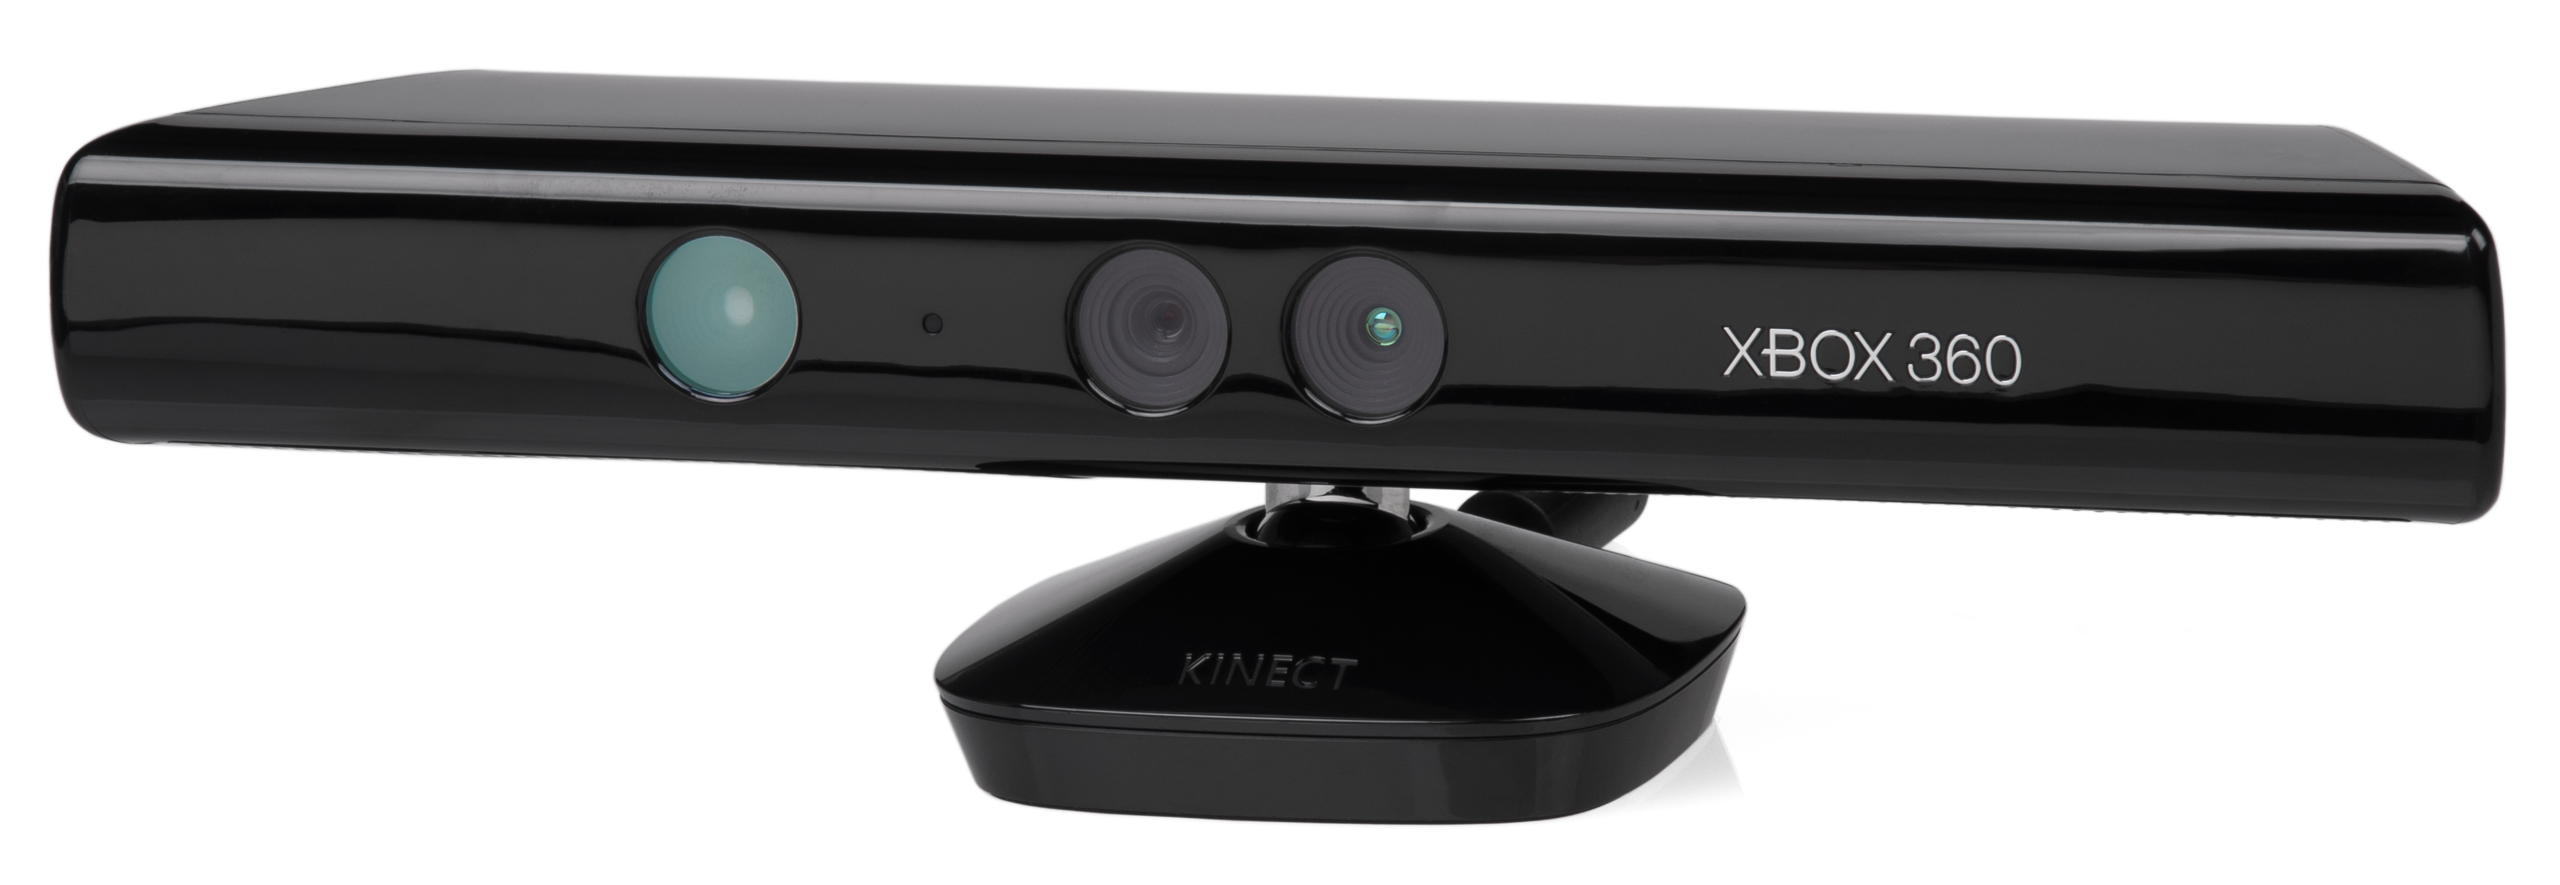
\includegraphics[width=0.45\linewidth]{figs/Xbox-360-Kinect-Standalone.png}(a)
	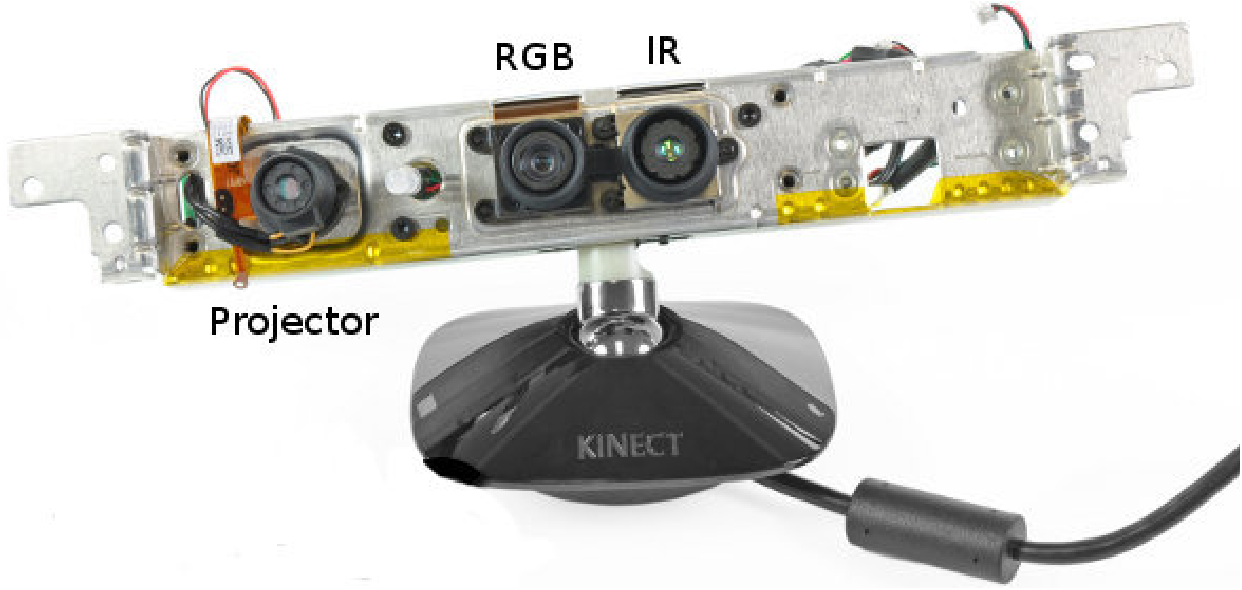
\includegraphics[width=0.45\linewidth]{figs/kinect-internals.pdf}(b)
 	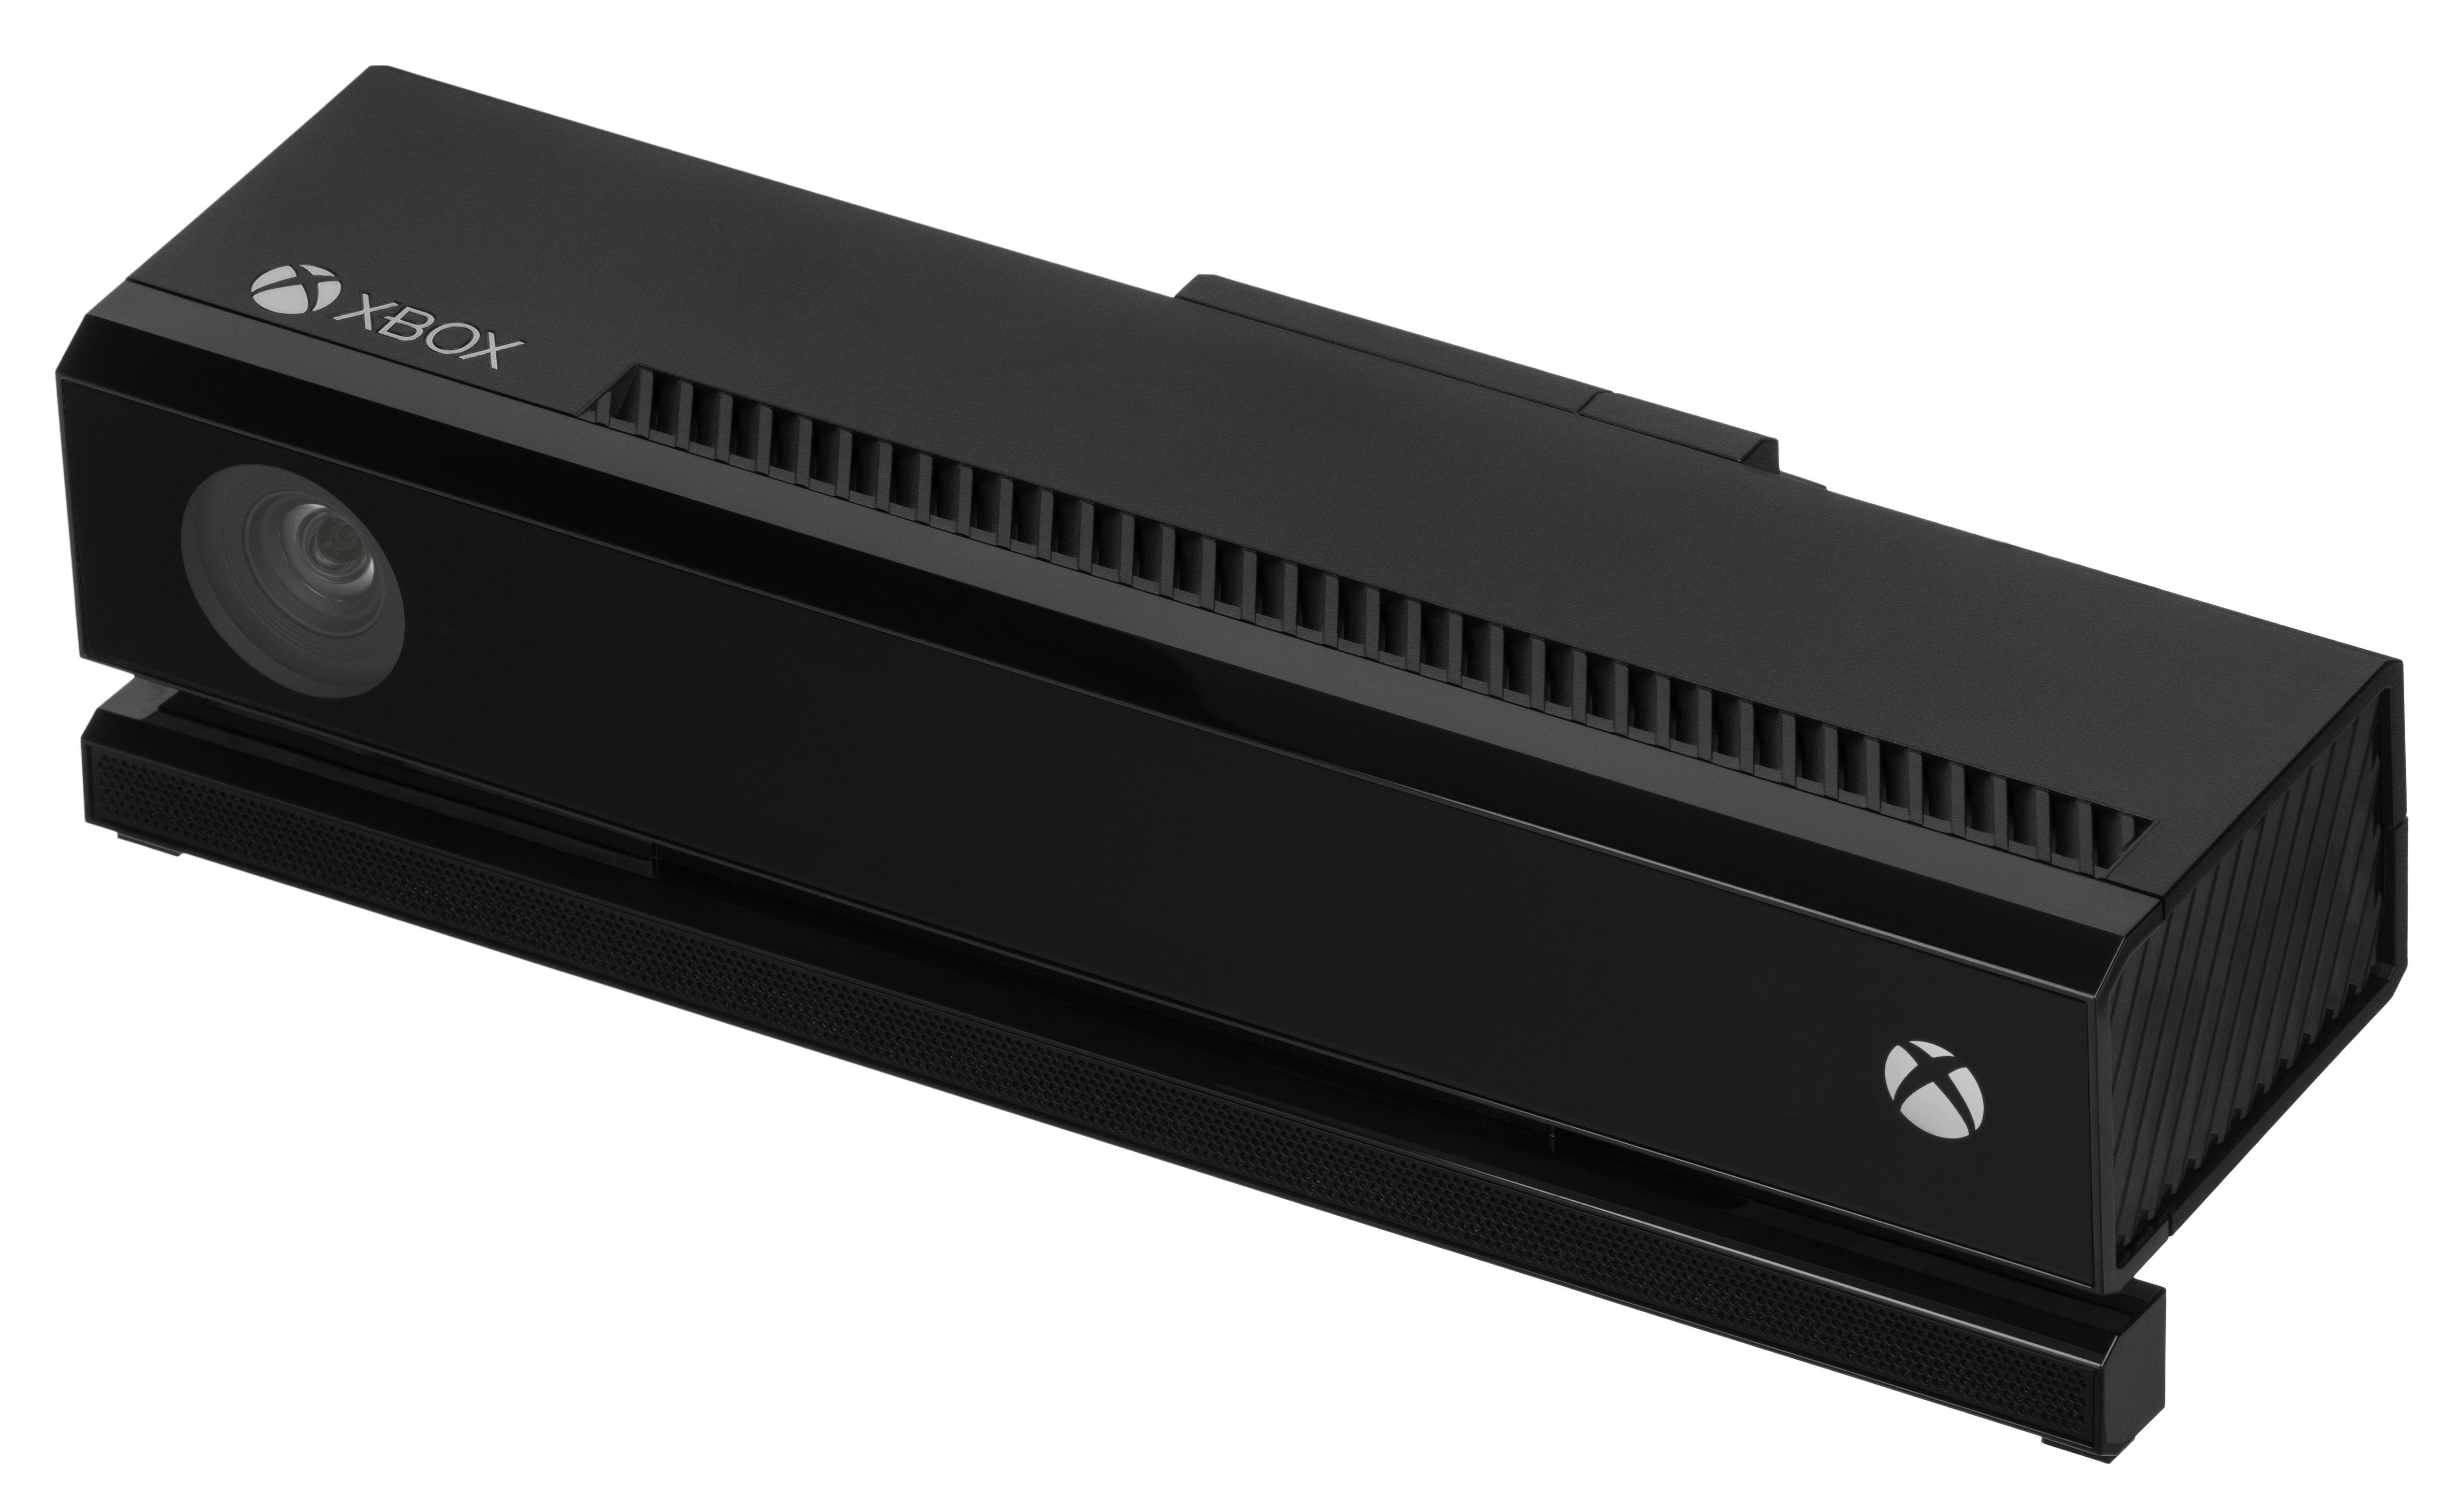
\includegraphics[width=0.45\linewidth]{figs/Xbox-One-Kinect.jpg}(c)
 	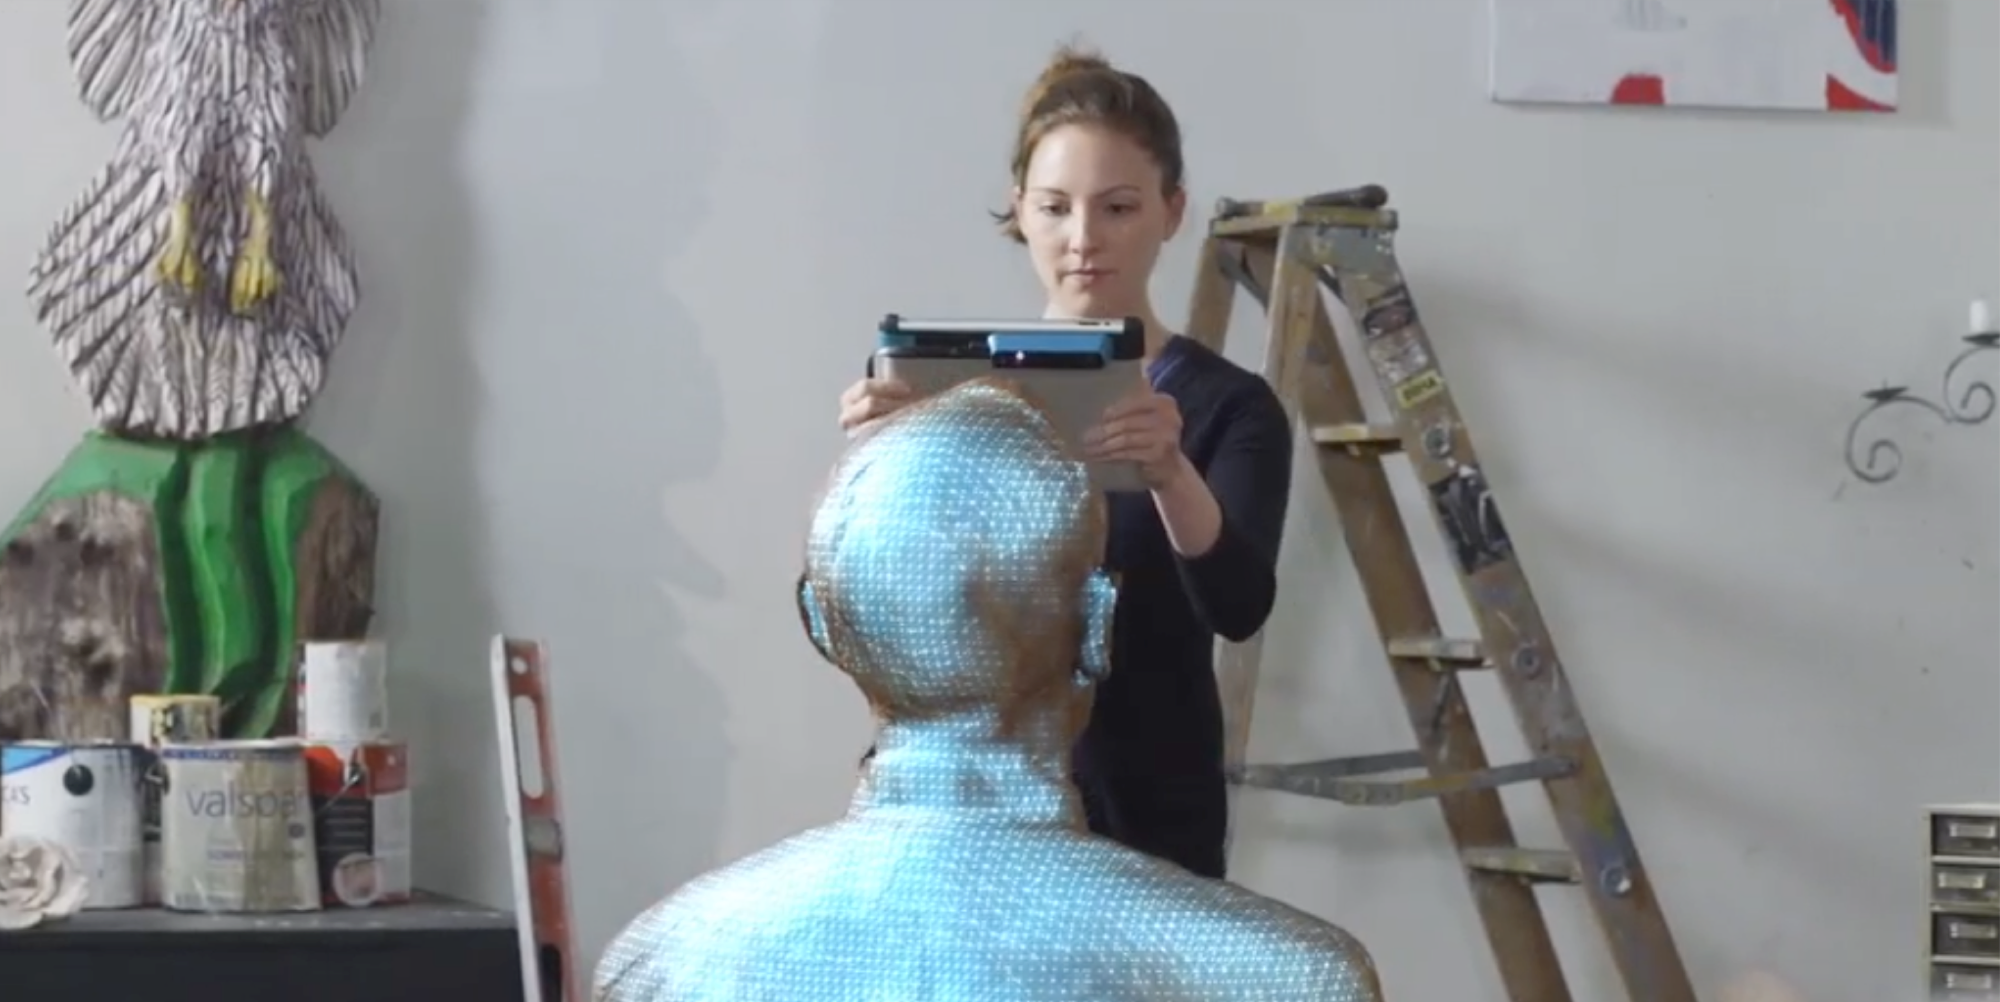
\includegraphics[width=0.45\linewidth]{figs/kinect-handheld1.png} (d)
	\caption{%
   Kinects de primeira geração (a) consistindo de câmeras e projetores
   infra-vermelho (b) e de segunda geração, consistindo de tecnologia ToF (c). 
   Ambos os kinects são largamente utilizados para escaneamento em tempo real, 
   formando a base de scanners manuais (d), porém nem sempre são úteis para 
   preservação detalhada de patrimônio. Um dos objetivos deste
   projeto é explorar os limites desta tecnologia.
	}\label{fig:kinect}
\end{figure}

A preservação de patrimônio tem sido realizada tradicionamente com scanners
dedicados de alto custo, como no projeto David~\ref{fig:david}.
O projeto teve início em 1992 e tem como objetivo a utilização de scanners a laser de profundidade
({\it rangefinder scanners}), aliado com algoritmos que combinam diferentes profundidades e cores da imagem, 
para realizar uma digitalização da parte externa e da superficie de forma acurada da estátua de David 
(porém, esse método pode ser utilizado em diferentes objetos no mundo real, 
como partes de máquinas, artefatos culturais e na indústria de video games, por exemplo). 
Para as partes mais detalhadas, foi utilizado um scanner de menor escala que faz uma pequena 
triangulação com laser de profundidade.

Seria de grande interesse explorar os dois paradigmas supracitados
para avaliar as possibilidades disponíveis no estado da arte de reconstrução 3D
para o escaneamento de baixo custo para a preservação de Patrimônio. O que se
pode atingir com apenas uma filmagem de esculturas realizada por um smartphone,
sem calibração prévia e \emph{in situ}, ou seja, sem ambiente controlado?  Como
esta recontrução se compara nos dias de hoje com a reconstrução realizada por um
scanner padrão baseado em Kinect?

\begin{figure}[!h]
	\centering
	%   \includegraphics[width=1.0\linewidth]{figs/3d-curve-sketch/system-diagram.eps}
	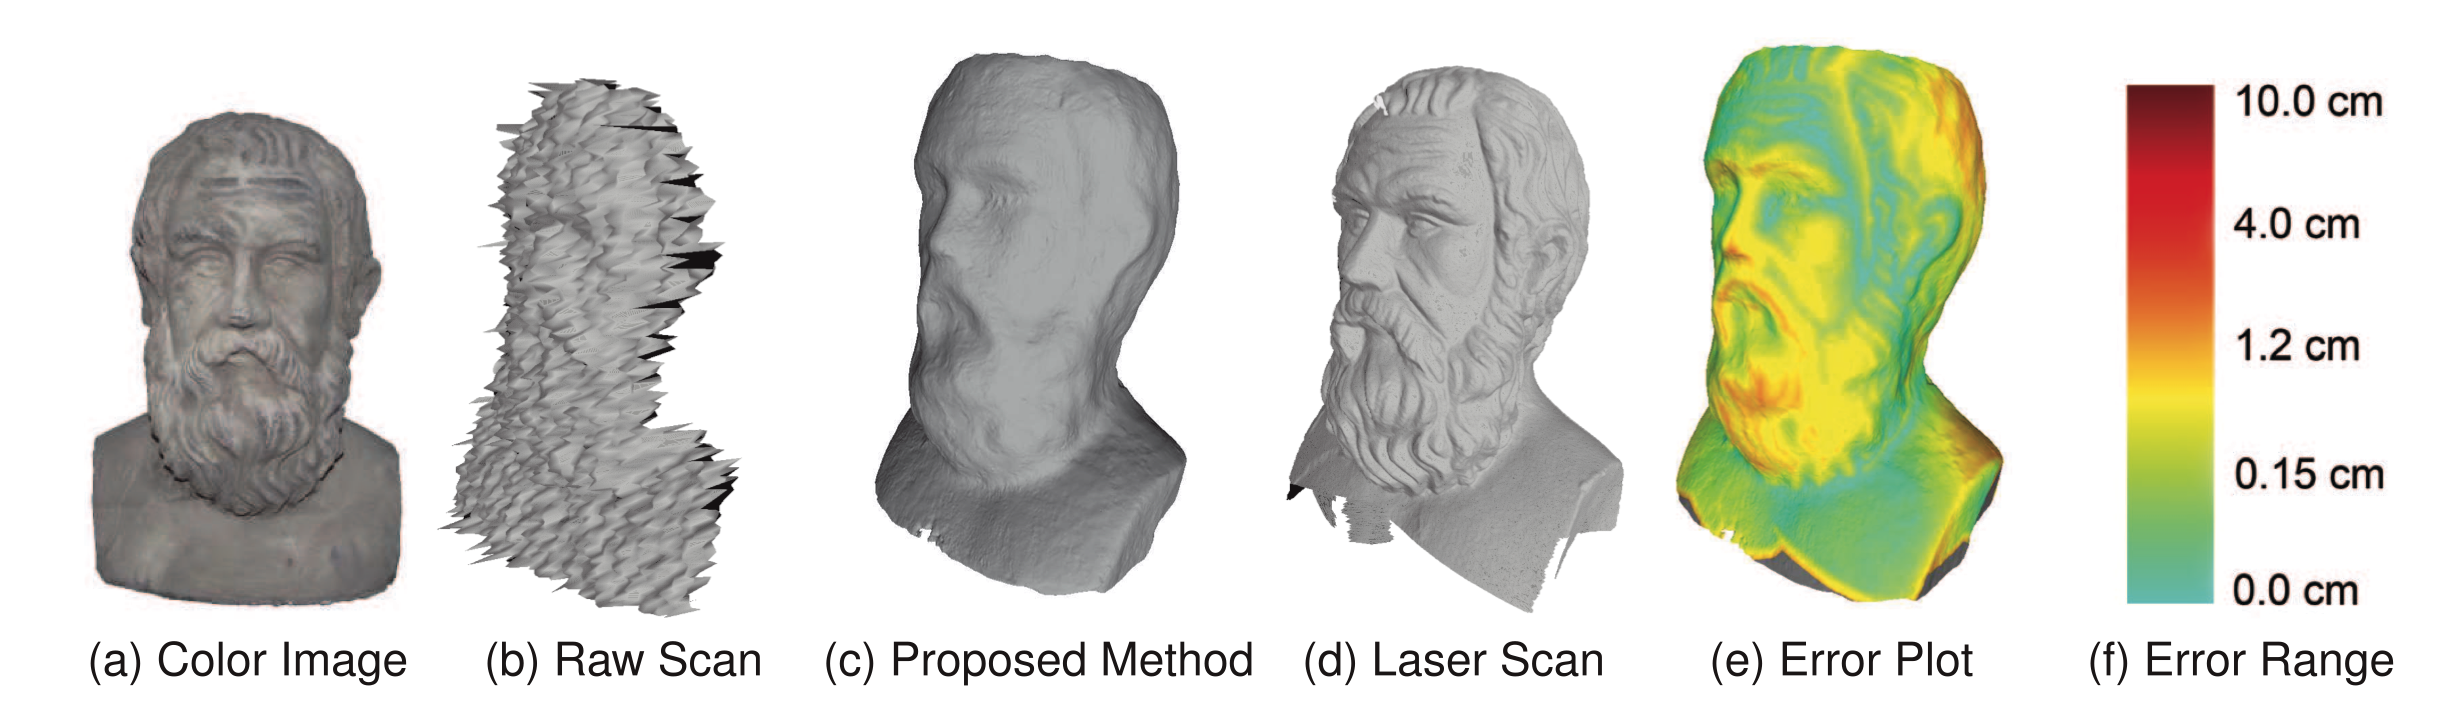
\includegraphics[width=1\linewidth]{figs/kinect-vs-usual.png}
	\caption{%
    A reconstrução usando-se Kinect (de primeira ou segunda geração) usando
    software atual de super-resolução (c) fornece precisão similar a um sistema estéreo de média
    resolução, inferior um sistema a laser de alta qualidade (d) porém de baixo custo e
    muito mais versátil devido ao sistema de aquisição manual e a software
    amplamente utilizado e
    desenvolvido\cite{wang2015research}.
	}\label{fig:rec3d:comparacao}
\end{figure}

\begin{figure}[!h]

\centering

\subfloat[]{\label{fig:davida}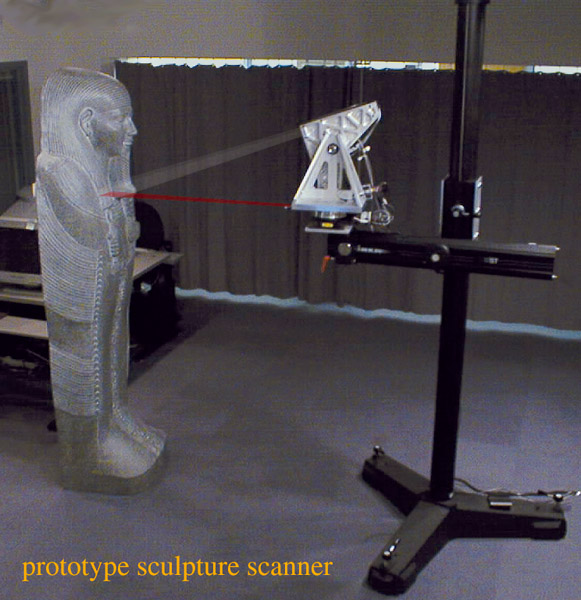
\includegraphics[width=0.18\linewidth]{figs/Proto+Inka+Egypt_light-s.jpg}}
% \vspace{2ex}
\subfloat[]{\label{fig:davidb}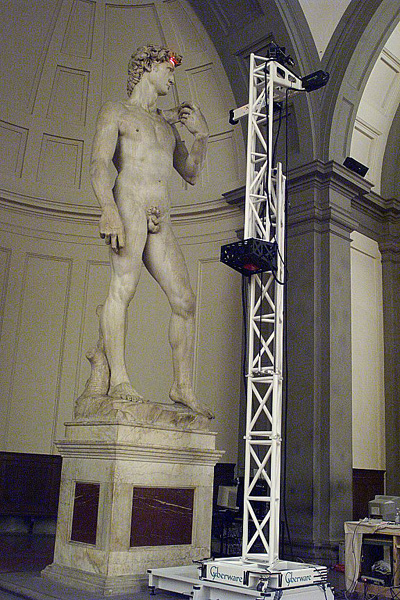
\includegraphics[width=0.18\linewidth]{figs/gantry-with-david-s.jpg}}
\subfloat[]{\label{fig:davidc}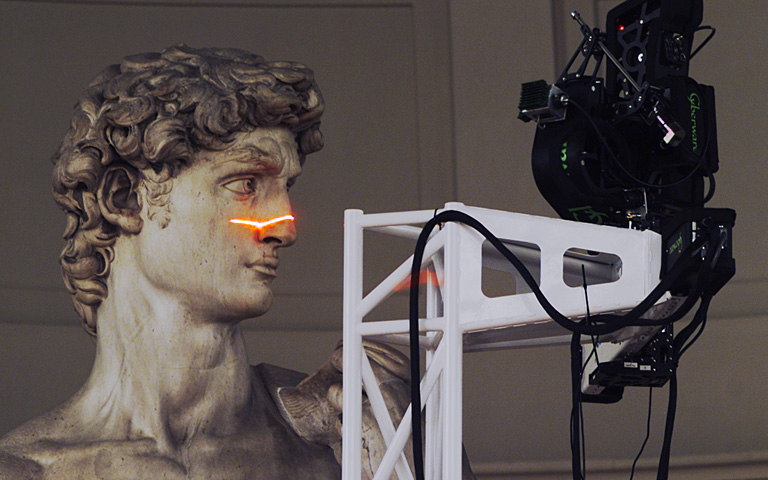
\includegraphics[width=0.18\linewidth]{figs/scanner-head-and-david-head-s.jpg}}
% \vspace{2ex}
\subfloat[]{\label{fig:davidd}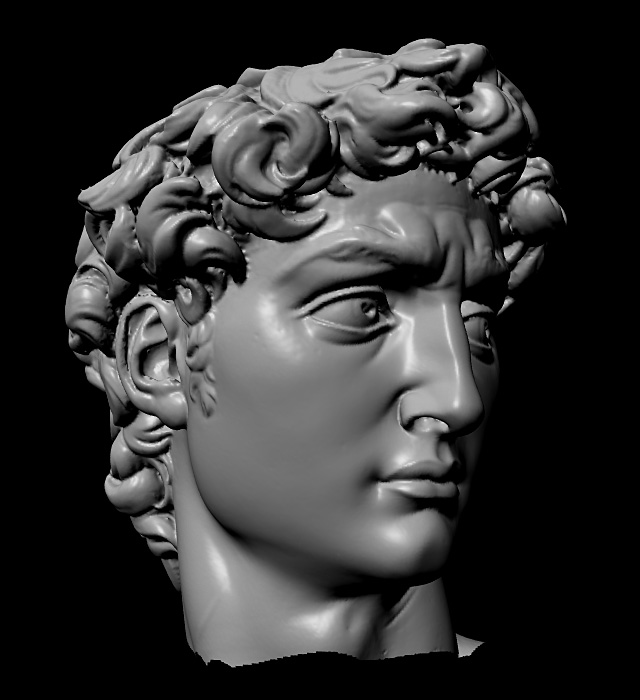
\includegraphics[width=0.18\linewidth]{figs/david-classic-leftlight-s.jpg}}
\caption{%
   Protótipo do scanner a laser de triangulação. O objeto a ser escaneado é uma réplica em tamanho real
   de um sarcófago egípcio (a). O scanner foi reconfigurado para escanear objetos maiores, pois 
   a escultura possui 517 centímetros (b), o da cabeça também sofreu uma reconfiguração, este scanner gira em 90 graus, 
   que faz o laser rotacionar, da posição horizontal para a vertical e também roda em torno da cabeça como um todo (c).
   Para a reconstrucão, o primeiro passo foi alinhar cerca de 100 scans em diversas posicoes, após isso, utilizado um 
   alinhamento automatico em pares dos scans, utilizando um algoritmo modificado de iteracoes de pontos próximos 
   (ICP - \emph {iterated-closest-points}). Após isso, faz-se um processo de relaxação global a fim de minimizar erros 
   de alinhamento por toda a estátua. Depois de alinhados, usa-se o algoritmo de profundidade volumétrica de 
   processamento de imagens (VRIP - \emph {volumetric range image processing} - do Brian Curless) (d).
	}\label{fig:david}
\end{figure}

\subsection{O Jardim do Nêgo, Nova Friburgo}
No caso de Nova Friburgo, há a necessidade redobrada de preservação do
patrimônio, em especial devido às chuvas e deslizamentos inerentes à região.  O
Jardim do Nêgo consiste em grandes esculturas em encostas, cobertas por um tapete de
vegetação, as quais desfrutam de grande reconhecimento regional e internacional~\cite{JardimDoNego:TheGuardian},
figura~\ref{fig:esculturas}.

\begin{figure} [!h]
	\centering
	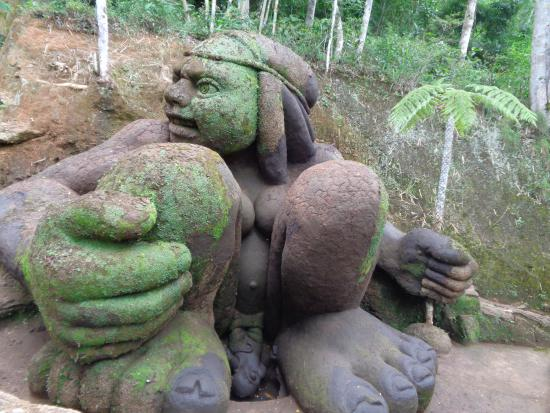
\includegraphics[width=0.3\linewidth]{figs/jardim-do-nego.jpg}
	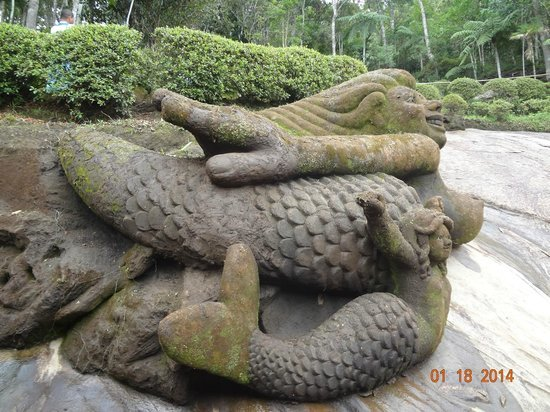
\includegraphics[width=0.3\linewidth]{figs/jardim-do-nego22.jpg}
	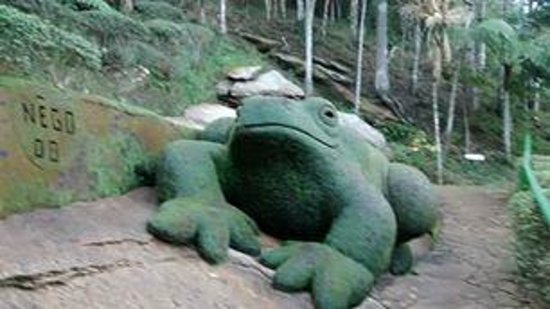
\includegraphics[width=0.35\linewidth]{figs/jardim-do-nego32.jpg}
	\caption{Algumas esculturas do Jardim do Nêgo}\label{fig:esculturas}

\end{figure}


\begin{figure} [!h]
	\centering
	%   \includegraphics[width=1.0\linewidth]{figs/3d-curve-sketch/system-diagram.eps}
	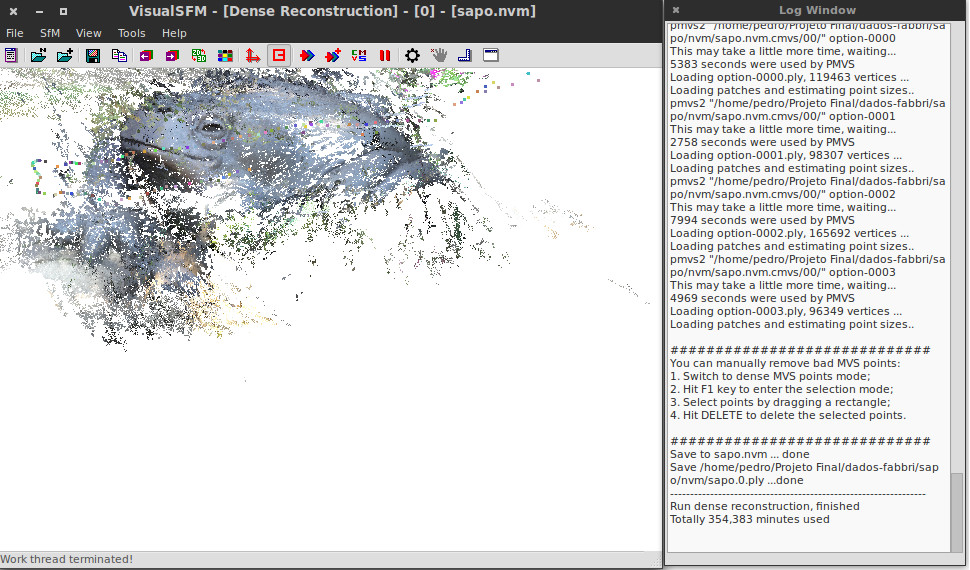
\includegraphics[width=1\linewidth]{figs/rec3d.jpg}
%	\includegraphics[width=0.95\linewidth]{figs/rec3d-curves-pmvs.pdf}
	\label{fig:rec3d}
	\caption{A reconstrução usando-se apenas imagens, sem controle de aquisição, 
	   como em um vídeo de um smartphone filmado em torno do objeto, fornece uma
	   nuvem de pontos, que pode ser
	   densificada~\cite{snavely2010bundler,wu2011visualsfm,furukawa2007dense,mve}, ou
	   atribuída de
	   curvas~\cite{Usumezbas:Fabbri:Kimia:ECCV16,Fabbri:Kimia:IJCV2016,Fabbri:Kimia:CVPR10,Fabbri:Giblin:Kimia:ECCV12}, de forma a preservar a resolução
	   em áreas de alto conteúdo informativo. Tais representações estão sendo
	   atualmente unificadas na pesquisa da área. Este projeto propõe explorar os
	   limites da reconstrução 3D usando-se apenas imagens, no contexto de
	   preservação de patrimônio.}
\end{figure}


Idealizado e criado por Geraldo Simplicio (Nêgo), artista cearense que mora no 
local a mais de 30 anos, ganhou notoriedade por suas esculturas de barro, com traços 
singulares e técnicas únicas. Hoje, trabalha para reconstruir o Jardim da tragédia de 
2011 na região serrana, onde algumas estruturas foram destruídas. Portanto, com o 
consentimento do Nêgo, surgiu a motivação desta pesquisa: além de explorar métodos de 
reconstrucão, também tem o objetivo de eternizar um patrimônio que é reconhecido no mundo
todo.

A preservação das esculturas do Jardim do Nego se torna um desafio à pesquisa em
recontrução 3D, pois apresentam curvas bem delineadas, que são 
representadas de maneira suavizada e empobrecida por métodos convencionais.
Algumas esculturas apresentam pouca textura, quase sem nenhum padrão de textura/musgo.
Seria de grande interesse availiar o potencial de técnicas atuais de
reconstrução 3D geral sem controle de aquisição, as quais têm seu código fonte
disponível na internet.

\section{Objetivos}

O presente projeto pretende fazer com que o aluno ganhe experiência com técnicas
modernas de reconstrução 3D fotogramétrica, no contexto de uma aplicação
bem-definida de preservação de patrimônio. A entrada do sistema deverá ser um
conjunto de vídeos realizados por câmeras de baixo custo, ou um conjunto de
escaneamentos realizados por scanners à mão de baixo custo baseados em Kinect.

O objetivo concreto do aluno será explorar as tecnologias supracitadas para
desenvolver um esquema de escaneamento usando software aberto, câmeras e
scanners de baixo custo, representando o estado da arte em reconstrução 3D sem
restrições de aquisição. Perguntas fundamentais a serem respondidas são: que
nível de detalhe, facilidade e precisão se pode obter usando-se apenas imagens e software
aberto? É possível utilizar scanners de baixo custo baseados em Kinect com
melhorias significativas em termos de qualidade, conveniência ou tempo de
processamento?  Quais são as restrições desses sistemas? Seria útil na prática
uma reconstrução de curvas para auxiliar na reconstrução de nuvem de pontos e de
superfícies densas? Onde o estado da arte deve ser avançado de forma a permitir
uma solução mais conveniente e completa para a preservação de patrimônio?

O principal objetivo em termos de pesquisa científica será comparar as
diferentes abordagens do estado da arte disponíveis para reconstrução 3D e
explicitar suas limitações práticas. O aluno deverá, com o entendimento das
abordagens, desenvolver um esquema de aquisição de esculturas que permita
ampliar os detalhes ou ajudar a resolver os problemas dos métodos. Com a
experiência obtida, o aluno estará pronto para desenvolver pesquisa futura na
área de recontrução 3D, com conhecimento de causa para avaliar direções de
pesquisa de efetivo e alto impacto na prática.

\section{Organização deste manuscrito}

O trabalho foi estruturado da seguinte maneira: previamente introduzimos os métodos baseados em pontos de interesse no Capítulo~\ref{sec:pontosdeinteresse}, destacando suas funcionalidades. No Capítulo~\ref{sec:denserecon} discutimos e aprofundamos o  funcionamento de cada algoritmo de reconstrução densa empregados, apresentando e debatendo, comparativamente, pontos à favor e contra; O Capítulo~\ref{sec:kinect} é apresentada a técnica de reconstrução utilizada nos  {\it Kinects}, da Microsoft; Com isso, temos o  Capítulo~\ref{sec:visualsfm}, que é dedicado à ferramenta gráfica utilizada para a obtenção dos resultados (VisualSfM) dos algoritmos de reconstrução densa utilizados. Finalmente, apresentamos os resultados e conclusões do trabalho, bem como sugestões para implementações e trabalhos futuros.
%Este trabalho está organizado da seguinte forma: discutimos as técnicas de
%extração de curva sem aprendizagem de máquina supervisionada no
%Capítulo~\ref{sec:cfrag:extraction}. No Capítulo~\ref{sec:learning:chapter},
%discutimos maneiras pelas quais essas técnicas podem ser melhoradas
%usando dados de treinamento anotados por humanos como entrada para uma
%aprendizagem de máquina geométrica de topologia e semântica de fragmentos de
%curva. A maior parte deste material é
%de~\cite{Guo:etal:CVPR14,Guo:etal:PAMI2017:submitted,Tamrakar:PHD:2008}, com esclarecimentos
%substanciais e comentários sobre as questões relativas aos nossos objetivos
%específicos. No Capítulo~\ref{sec:generic:datasets}, apresentamos o processo de
%captura de dados confiáveis (\emph{ground-truth}), comparando os conjuntos de dados anteriores com o problema proposto
%neste trabalho para a água. Nos capítulos restantes, apresentamos e discutimos
%nossos resultados para vários vídeos em tanques de água. Partes deste trabalho
%foram apresentadas em~\cite{Fabbri:WaterWaves2016,Fabbri:WaterWaves2017,Souza:Fabbri:WaterWaves2017}.

%======================================================================================
